\chapter{系统软件下的初步评测}

在完成基本的功能正确性评估后,本项目尝试启动Linux操作系统。
因为该项目的最终启动目标KVM是一个基于Linux的Type2虚拟机管理系统
只有在启动Linux的基础之上,才能够启动虚拟机。
本章讲述启动操作系统时对软件所需的适配,以及软硬件联合调试是遇到的困难以及解决方案。

\section{操作系统的适配与启动}
关于目标适配的虚拟化软件Linux KVM,是一个开源的Type2虚拟机管理系统。
在RISC-V架构方面,已经存在初步适配后的软件——kvm-riscv\cite{github:riscv-kvm},
该项目主要包括启动KVM选项并适配RISC-V架构后的Linux源码及配置、包括kvmtool的根文件系统。
该套完整系统软件可以直接在RISC-V处理器模拟器(qemu、spike)中运行。

特别是kvmtool,这是是一个Linux的用户态程序。
可以通过使用它在命令行中直接使用KVM,在Linux中启动一个虚拟机。
需要手动编译该软件并将其放入根文件系统中,考虑到根文件系统应该尽可能小,尽可能简便。
因此根文件系统中并未包含动态链接的可执行程序的系统库,例如libc和libm。
为此,kvmtool需要被静态编译,特别是其依赖库libfdt,
也需要将其静态编译后,一起链接到kvmtool中。

本项目计划在FPGA中部署硬件直接启动Linux和KVM,通过观察串口输出判断是否正常运行。
因为完成操作系统的启动至少需要3亿以上的周期数,
逻辑软件仿真的速度太慢,需要花费数天的时间才能完成。
因此,需要让系统软件对FPGA平台的进行一定的适配:
编写对应平台专用设备树,还需要根据FPGA使用的外设开启对应的驱动。

完成软件适配之后,需要在FPGA上启动进行软硬件联合调试。
但是在尝试启动Linux时遇到了难以调试的问题:
Linux的输出停止在如图\ref{fig:console-block}所示的地方。
由于在FPGA运行无法获取波形图,难以观察电路内部的情况。
此时离上电复位也经过了数百万个周期,即使使用逻辑仿真也需要极长的时间才能运行到出错点。

\begin{figure}[htbp]
    \centering
    
\includegraphics[scale=0.6]{empty.png}
    \caption{虚拟化扩展后的“香山”启动Linux的串口输出}
    \label{fig:console-block}
\end{figure}

为了能够快速仿真到出错点,并且使用逻辑仿真软件生成波形的能力观察电路内部细节,
本项目使用REMU\cite{iccd2023remu}——基于FPGA的仿真加速平台,进行调试。
平台的实物图如\ref{fig:remu-card}所示。
通过使用REMU,可以在FPGA中快速地将Linux启动到任意时刻,然后使用ctrl-c中断现场,
并将此时硬件内部所有寄存器和存储器通过检查点的方式保存。
检查点数据通过DMA从FPGA发送到x86主机后,
可以被逻辑仿真软件工具重放,即可快速地得到数百万周期后的波形。



\begin{figure}[htbp]
    \centering
    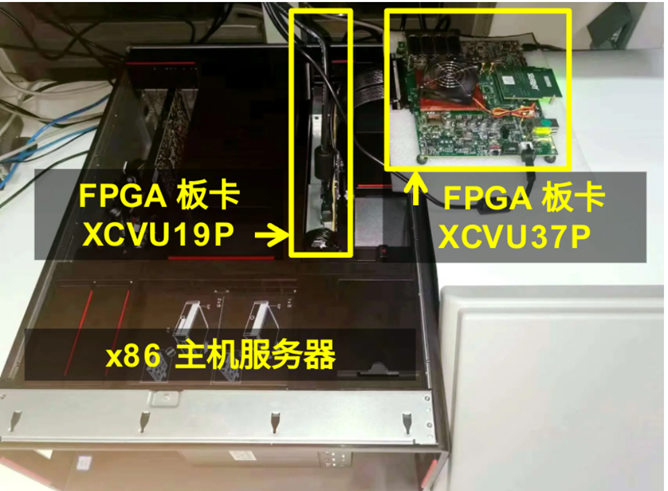
\includegraphics{remu-card.png}
    \caption{REMU平台硬件实体}
    \label{fig:remu-card}
\end{figure}

通过观察如图\ref{fig:console-block-wave}所示的REMU重放波形,
可以清楚地观察到处理器在某一时刻后没有提交任何的指令,也没有对外发起任何的访存请求。
造成这种现象的一般原因是某一级流水线的自动机设计缺陷:
某种特殊情况使得状态机停滞在某一状态,无法进行状态切换,导致整个处理器停滞。
经过细致的波形分析即可发现,是指令缓存的状态机设计的缺陷。
在某种特殊的不命中的情况下,既不对外发起访存请求,也不使用内部缓存块数据返回。
在REMU的帮助下,找到了错误的代码进行修改后,Linux能够正常启动。

\begin{figure}[htbp]
    \centering
    
\includegraphics[scale=0.6]{empty.png}
    \caption{REMU重放的Linux启动波形}
    \label{fig:console-block-wave}
\end{figure}

\section{操作系统下的性能评测}
在多年发展下,虚拟化评测已成为一个研究良好的领域,开发了许多评估各种虚拟化平台性能的基准方法。
可以根据粒度将现有的基准大致分为微观基准和宏观基准。
宏观基准评估实际应用程序在松散定义的条件下的整体性能,
如lmbench、SPEC CPU 2006等。
微基准测试衡量的是在定义良好的条件下单个原始操作的性能。
但是不论是宏观还是微观,其中一个重要的基准线便是主机性能,即未开启虚拟化下的运行基准测试的性能。
该阶段已经完成Linux操作系统的启动,在评估虚拟化性能前,可以先对主机性能进行简单评测。
于是,同样在FPGA平台中,使用虚拟化扩展的“香山”处理器,启动Linux。
在Linux中,通过命令行运行CoreMark、Dhrystone等基准测试。
同时,作为对比也使用了未添加虚拟化扩展的“香山”处理器进行,对比结果如图\ref{fig:perf}所示。
根据测试结果可以看出,虚拟化扩展的添加,对主机性能影响并不大,保持了原有的高性能乱序核的特点。

\begin{figure}[htbp]
    \centering
    
\includegraphics[scale=0.6]{empty.png}
    \caption{虚拟化扩展后的“香山”与原始“香山”的性能对比}
    \label{fig:perf}
\end{figure}

\chapter{虚拟机管理系统的调试}
通过对系统软件的修改移植,现阶段可以在添加虚拟化扩展的“香山”处理器中启动操作系统,
运行主机级别用户态程序,并对主机性能进行了简单的评测。
下一步需要运行虚拟机,并尝试在虚拟机中运行相同的用户态程序,以评测虚拟化性能。
本章描述在使用虚拟化扩展的“香山”运行KVM,其中遇到的难以调试的错误以及对调试方案的探索。

\section{虚拟机启动的现象}
在命令行工具中通过kvmtool工具,尝试启动虚拟机。
但是串口输出如图\ref{fig:kvm-run}所示,没有进一步虚拟机Linux启动的输出。

\begin{figure}[htbp]
    \centering
    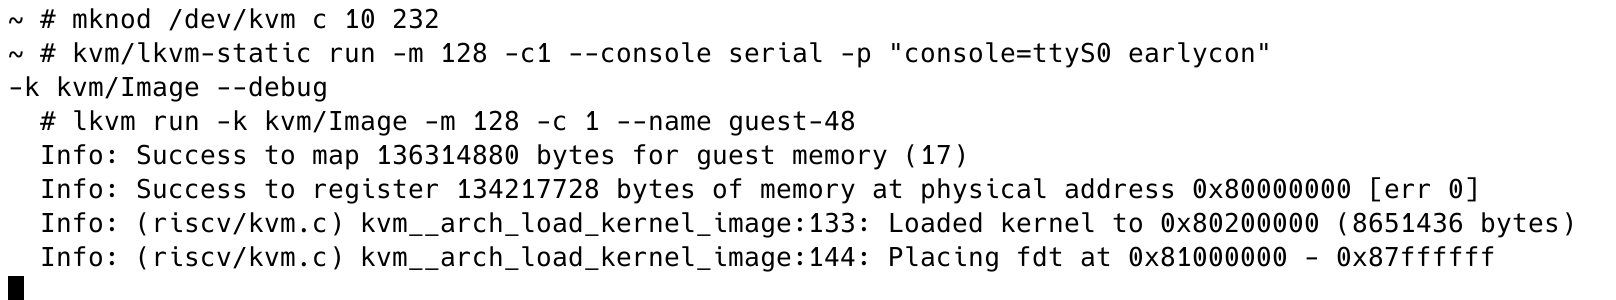
\includegraphics[scale=0.35]{kvm-run.png}
    \caption{使用kvmtool启动虚拟机的串口输出}
    \label{fig:kvm-run}
\end{figure}

为了观察电路内部状态,使用REMU重放此刻的波形。
波形如图\ref{fig:kvm-wave}所示,从中可以看出如下所示的一些现象:
\begin{itemize}
    \item 指令提交没有停止,在正常流动
    \item 指令的虚地址位于\verb|1FF_800X_XXXX|区域,物理地址位于\verb|802X_XXXX|区域
    \item 处理器目前运行在虚拟机监管模式,尚未开启虚拟位
    \item 控制状态寄存器satp.mode值为8,代表第一阶段地址翻译正常开启
\end{itemize}
尽管可以从波形中获取更多的体系结构、甚至是微架构信息,但是对调试帮助甚微。
因为调试不仅需要此刻已有的硬件的体系结构信息,还需要此刻正确的体系结构信息应该是什么。
通过比对正确和已有的体系结构信息,才能一步步反推出错原因。
换言之,只有找出体系结构信息出错的现场、甚至是第一现场,才能帮助处理器调试。
但此时距离处理器上电复位已经运行了49亿以上的时钟周期,此时处理器的内部状态十分复杂。
在该时间点处理器的的正确的体系结构信息应该是什么,是一件很难确定的事情。
一方面,无法知道处理器在运行软件的哪一部分。
可能是系统软件、也可能是被加载到内存中的应用程序。
后者将极大的增加软硬件联合调试的难度,因为虚拟地址的使用,导致加载地址是可浮动的。
此外,仅仅知道执行的汇编代码对调试帮助不大,了解汇编对应的源码部分的语义才能更快调试错误。
另一方面,纵使知道了“香山”处理器在执行当前系统的软件的哪一部分,
也很难获取此时处理器内正确的体系结构信息。
尽管可以使用其他的处理器,或者是模拟器运行相同的系统软件,并停止在该部分。
但是执行中所需的外设输入,访存延时等各种不确定信息需要被精确重放在其他的处理器中,
才有可能保证两个处理器对同一系统软件的执行路径是相同的,得到可用的、正确的的体系结构信息。
综上所述,为了调试错误,当务之急是找到一种既能精确定位错误现场,又能通过仿真快速迭代的调试手段。

\begin{figure}[htbp]
    \centering
    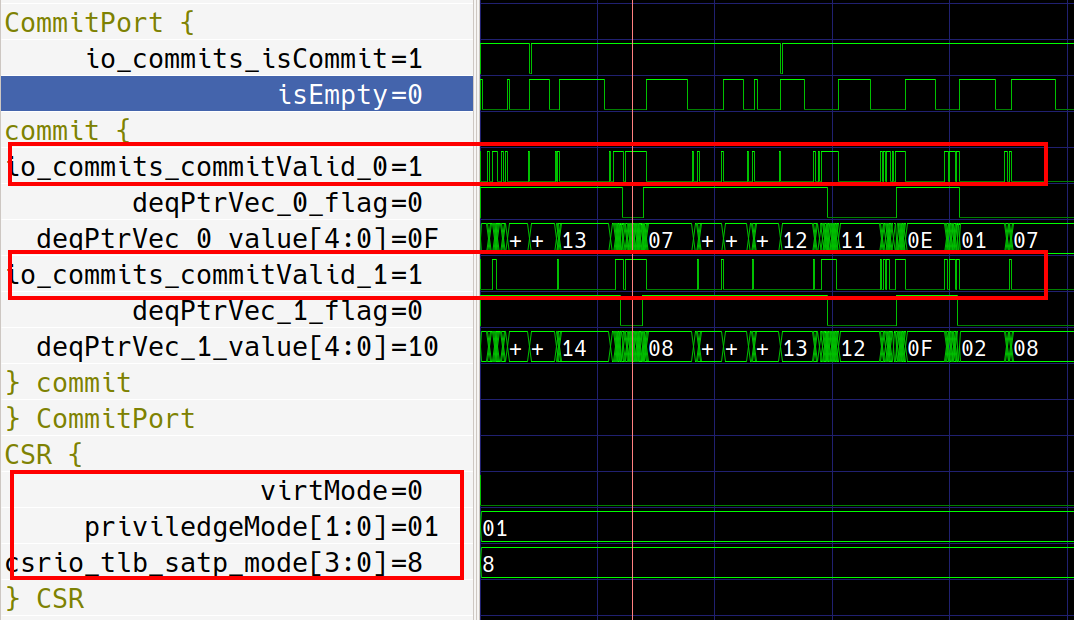
\includegraphics[scale=0.5]{kvm-wave.png}
    \caption{使用kvmtool启动虚拟机的串口输出}
    \label{fig:kvm-wave}
\end{figure}

\section{现有调试手段的限制}
现阶段,“香山”处理器官方调试方法依然是纯软件仿真和差分测试。
通过实时比对“香山”处理器和处理器模拟器NEMU的体系结构信息,
并在一些关键的时刻,例如中断、外设输入等,让“香山”指导模拟器的执行路径。
从而保证了在任意时刻,“香山”处理器的体系结构信息是正确的。
一旦在体系结构信息层面出现微小的错误,差分测试框架会立刻停止仿真、汇报错误。
然而,逻辑仿真软件的速度是不可接受的。
为了调试上述错误,尝试使用差分测试框架进行逻辑仿真。
结果从上电复位开始进行逻辑仿真,花费两天时间仍然无法完成Linux的启动。
更不必说还需要通过串口进行命令行的输入kvmtool启动虚拟机。
由此可见,尽管软件仿真能够精确的定位错误现场,速度是最主要的限制。

另一方面,FPGA的加速仿真框架REMU,
虽然可以使用FPGA加快仿真的速度,并在逻辑仿真软件中精确地重放波形。
但是仅作为一个仿真框架,无法提取体系结构信息、
并实时和正确的体系结构信息进行比对,也就难以精确地定位错误现场。
对REMU而言,最主要的限制在于其灵活性、也就是使用方式。
因为只有在部分特殊的情况下,即可以从波形明显看出出错现场的时刻,
波形重放工具才能够独立的完成错误调试的任务。
在大部分情况下,包括目前遇到的问题,尚不足以解决。
为了调试KVM运行卡住的原因,仅存在重放波形唯一的使用方法。
但通过波形重放,无法明显的看出具体问题。
不同于单纯的硬件卡死卡住,此时指令一直流动、不知道处理器在运行软件的哪一部分。
一旦脱离了体系结构信息,处理器调试会变得毫无根据。
为此REMU在处理器调试方面,急需一套完整能够提取体系结构信息的基础设施。

\section{潜在调试方案的探索}

\paragraph{逻辑仿真软件}
上述提到软件仿真的主要限制是速度,从上电复位开始仿真到操作系统启动所需的时间很长。
那可以考虑从操作系统启动之后开始仿真,跳过已经能够正确运行的操作系统启动部分。
“香山”官方的配套基础设施也有类似的支持。
他们为NEMU,“香山”专用的处理器模拟器,添加了生成检查点的功能。
NEMU可以在运行任意负载的任意时刻停下,将此刻的体系结构信息保存成检查点。
这里描述的检查点,是此时NEMU执行至此的内存布局。
同时还在内存指定的地方,存储所有的体系结构寄存器信息。
在“香山”处理器进行逻辑仿真的时刻,会先执行一段汇编。
通过访存指令,从内存指定的地方加载所有的寄存器的数值到对应的体系结构寄存器中。
之后使用跳转执行继续检查点的下一条指令。

换言之,使用“香山”官方提供的检查点方法,
能够把启动完操作系统的处理器的体系结构信息放入“香山”后,再启动仿真。
但是对于微架构寄存器则无能为力,
因为既不存在、也没必要存在一个和“香山”微架构一模一样的模拟器。
尽管这种方法可以复现部分错误,
但是对于类似数据缓存、页表缓存、页表翻译单元等没有任何体系结构信息的单元,
无法复现错误的概率也很大。
缓存单元的错误很可能在上电复位之后会被隐藏,正是在持续运行中才有可能暴露。
尽管如此,不论是否能发现错误,本项目中依然尝试了该方法进行处理器的调试。
然而在系统软件的适配中遇到了问题,由于时间限制,尚未完成调试。
关于系统软件的问题,由于NEMU和“香山”的SoC在启动时暂时不支持外存。
所以根文件系统必须要和内核镜像打包在一起。
然而尝试使用NEMU单独启动操作系统之后,如图\ref{fig:init-block}所示无法完成init进程的启动,进入Shell。
为了解决该问题,下一步需要使用QEMU和gdb进行联合调试,解决软件中潜在的问题。

\begin{figure}[htbp]
    \centering
    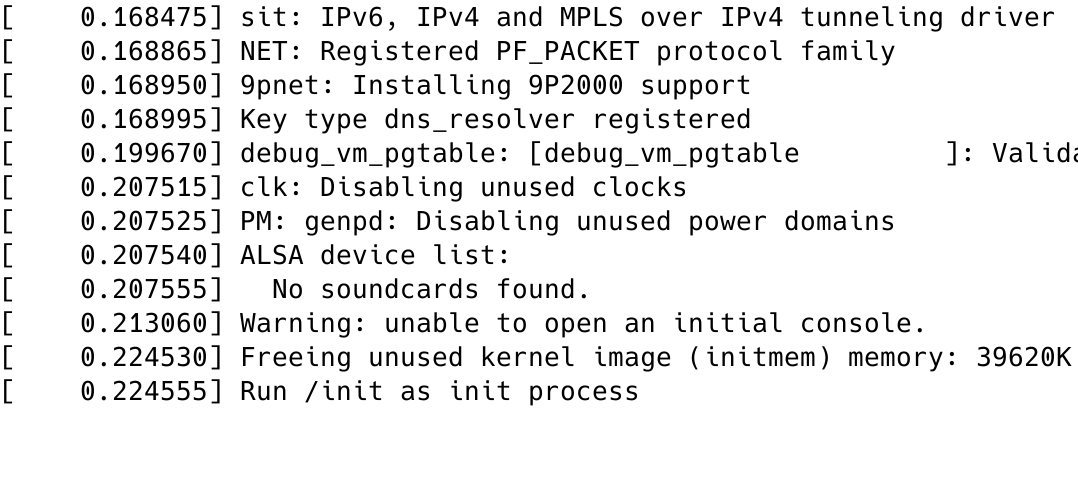
\includegraphics[scale=0.5]{init-block.png}
    \caption{NEMU启动Linux时无法完成init进程的加载}
    \label{fig:init-block}
\end{figure}

\paragraph{FPGA平台}
关于FPGA硬件加速仿真平台REMU,目前的检查点和波形重放功能十分单一,支持的逻辑仿真软件只有iverilog。
纵使想要使用REMU生成的检查点,重放到差分测试的仿真框架中这也是做不到的。
差分测试的仿真框架目前仅支持verilator和Synopsys VCS两种逻辑仿真工具。
分别是目前开源社区和商业界最高效的仿真工具,可配置程度高,仿真激励部分使用C++语言编写。
相比之下iverilog是更偏向教学与学术研究的工具,上手难度较低,
仿真激励部分使用verilog语言编写;相对的,在仿真速度和可配置程度上无法和verilator相比。
为了能让REMU的检查点发挥更大作用,支持verilator是一个必经之路。

为了将检查点数据放入逻辑仿真软件中,
REMU使用了verilog的语言规范中定义的编程接口:Verilog Procedural Interface(VPI)。
VPI作为一个语言规范,在iverilog和verilator中均有不同程度的部分实现。
然而对于重放检查点而言,仅仅需要满足向物理寄存器写入数据这一需求。
iverilog和verilator均存在对应的VPI实现,因此存在部分可复用的代码。
所需做的是使用C++编写verilator的仿真激励,修改部分verilator和iverilog不兼容的部分。
尽管目前已经能够使用verilator重放REMU检查点,但是在实用化上还远远不够。
后续还需要对接差分测试的仿真框架与目前已有的verilator仿真框架。
包括把检查点的数据放入模拟器NEMU在差分测试的仿真激励脚本中添加VPI的相关代码等。
该部分虽然仅只是作为工程实现,没有太多的设计创新的部分。
但是为REMU丰富了使用的方法,为后续REMU的差分测试硬件化打下基础。

仅仅实现逻辑仿真软件重放检查点数据是不够的,REMU需要更为精确的定位错误现场的方法。
可以考虑将差分测试的部分逻辑固化在FPGA中,同时利用FPGA的快速和差分测试的精准。
具体的固化实现是将FPGA中对应各种架构寄存器的物理寄存器、差分测试的使能信号等,
通过硬连线拉出到顶层,每周期进行采样。
对于需要比对的数据,则以DMA的形式从FPGA发送相连的到x86对应和模拟器进行比对。
这种差分测试硬件化的想法尽管在REMU平台发布时已经提出,
并对NutShell——国科大学生设计的简单乱序核,进行了适配,
但是对于“香山”处理器还未达到可用的地步,还需要进一步修改。
除了可用性的适配之外,还需要考虑的一部分则是处理速度,
需要完全精确地硬化差分测试中,FPGA每周期需要采样大量数据进行DMA,
DMA的传输速度和软件处理数据的速度会逐渐成为FPGA加速仿真的瓶颈。
因此需要精心设计需要传输数据的格式,或者降低比对的频率、多条指令提交后才进行一次比对。
其本质都是减少数据传输量,降低DMA和软件侧的负荷。
该部分的工作也因为时间限制尚未完成,会在今后成为研究方向。